% ============================================================================
% CHAPTER I: OVERVIEW OF EMBEDDED SYSTEMS
% Academic & Technical Presentation (LaTeX Beamer)
% Widescreen 16:9, Latin Modern Font, Cyan Header Banner (#00A8E1),
% Two-column figure layouts, and Overleaf-ready structure.
% ============================================================================
\documentclass[aspectratio=169,11pt]{beamer}

\usepackage[utf8]{inputenc}
\usepackage[T1]{fontenc}
\usepackage{lmodern}
\usepackage{graphicx}
\usepackage{xcolor}
\usepackage{tikz}
\usepackage{booktabs}
\usepackage{tabularx}
\usepackage{array}
\usepackage{colortbl}

% ---------------- Color Definitions ----------------
\definecolor{bannerblue}{RGB}{0, 168, 225}    % Primary Cyan #00A8E1
\definecolor{darknavy}{RGB}{15, 34, 64}       % Heading Navy
\definecolor{cardbg}{RGB}{245, 248, 250}       % Light Card Shading
\definecolor{calloutbg}{RGB}{235, 246, 252}    % Callout Box Shading
\definecolor{rowalt}{RGB}{245, 249, 252}       % Alternating Table Row
\definecolor{bordergray}{RGB}{215, 230, 240}   % Border Gray

% ---------------- Beamer Template Configurations ----------------
\setbeamertemplate{navigation symbols}{}
\setbeamertemplate{background}{}

% STRICT FOOTER: Page number only in bottom right, no footer bar, text, or date
\setbeamertemplate{footline}{%
  \hfill{\color{gray}\footnotesize\insertframenumber}\hspace{0.5cm}\vspace{0.3cm}%
}

% Cyan triangle bullet point
\setbeamertemplate{itemize item}{\color{bannerblue}$\blacktriangleright$}
\setbeamertemplate{itemize subitem}{\color{bannerblue}\footnotesize$\blacktriangleright$}
\setlength{\leftmargini}{0.45cm}
\setlength{\itemsep}{0.22cm}

% Slide title command inside top cyan banner (18pt, bold, uppercase)
\newcommand{\slidetitle}[1]{%
  \begin{tikzpicture}[remember picture,overlay]
    \fill[bannerblue] (current page.north west) rectangle ([yshift=-1.15cm]current page.north east);
    \node[anchor=west, text=white, font=\bfseries\fontsize{18}{22}\selectfont,
      text width=0.92\paperwidth, inner sep=0pt]
      at ([xshift=0.6cm,yshift=-0.58cm]current page.north west) {\uppercase{#1}};
  \end{tikzpicture}%
  \vspace*{0.75cm}%
}

% Section Header command (14pt, bold)
\newcommand{\sectionheader}[1]{{\fontsize{14}{17}\selectfont\textbf{\color{darknavy}#1}}\par\vspace{0.15cm}}

\begin{document}

% ============================================================================
% SLIDE 1: TITLE SLIDE
% ============================================================================
\begin{frame}[plain,t]
  \begin{tikzpicture}[remember picture,overlay]
    \fill[bannerblue] (current page.north west) rectangle ([yshift=-2.3cm]current page.north east);
    \node[anchor=west, text=white, font=\bfseries\fontsize{22}{26}\selectfont,
      text width=0.92\paperwidth, inner sep=0pt]
      at ([xshift=0.8cm,yshift=-0.9cm]current page.north west) {CHAPTER I: OVERVIEW OF EMBEDDED SYSTEMS};
    \node[anchor=west, text=white!95, font=\fontsize{13}{16}\selectfont,
      text width=0.92\paperwidth, inner sep=0pt]
      at ([xshift=0.8cm,yshift=-1.7cm]current page.north west) {Foundations, Core Technical Characteristics \& The 5-Layer Software Architecture};
  \end{tikzpicture}
  \vspace*{2.0cm}

  \begin{columns}[c]
    \begin{column}{0.58\textwidth}
      \raggedright
      \sectionheader{Academic Courseware \& Technical Lecture}
      \begin{itemize}
        \item \textbf{Curriculum Scope:} Embedded Systems Engineering \& IoT Edge Computing.
        \item \textbf{Engineering Paradigms:} Deep hardware-software co-design, deterministic timing, and strict resource-constrained optimization.
        \item \textbf{Target Silicon Architecture:} 32-bit Microcontroller Core (ARM Cortex-M85 / Renesas RA8M1 MCU).
        \item \textbf{Implementation Standards:} C99/POSIX firmware patterns, Hard Real-Time OS, and modular layered architectures.
      \end{itemize}
    \end{column}
    \begin{column}{0.38\textwidth}
      \centering
      \includegraphics[width=0.85\linewidth,height=0.55\textheight,keepaspectratio]{images/fig_cover.jpg}
    \end{column}
  \end{columns}
\end{frame}

% ============================================================================
% SLIDE 2: TABLE OF CONTENTS
% ============================================================================
\begin{frame}[t]
  \slidetitle{Table of Contents}
  \raggedright
  \vspace{0.1cm}

  \begin{columns}[t]
    \begin{column}{0.48\textwidth}
      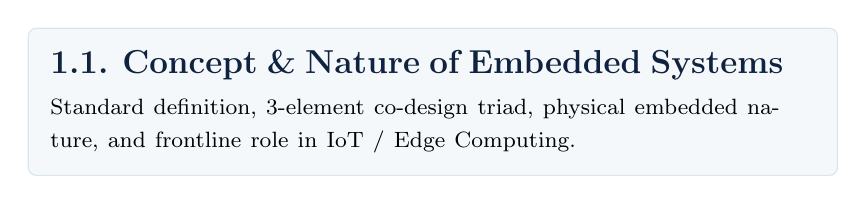
\begin{tikzpicture}
        \node[fill=cardbg, draw=bordergray, rounded corners=3pt, text width=0.45\paperwidth, inner sep=8pt] {
          \textbf{\fontsize{13}{15}\selectfont\color{darknavy}1.1. Concept \& Nature of Embedded Systems}\\[0.1cm]
          {\footnotesize Standard definition, 3-element co-design triad, physical embedded nature, and frontline role in IoT / Edge Computing.}
        };
      \end{tikzpicture}\\[0.25cm]
      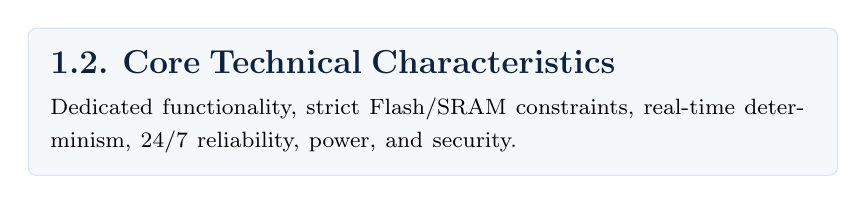
\begin{tikzpicture}
        \node[fill=cardbg, draw=bordergray, rounded corners=3pt, text width=0.45\paperwidth, inner sep=8pt] {
          \textbf{\fontsize{13}{15}\selectfont\color{darknavy}1.2. Core Technical Characteristics}\\[0.1cm]
          {\footnotesize Dedicated functionality, strict Flash/SRAM constraints, real-time determinism, 24/7 reliability, power, and security.}
        };
      \end{tikzpicture}
    \end{column}
    \begin{column}{0.48\textwidth}
      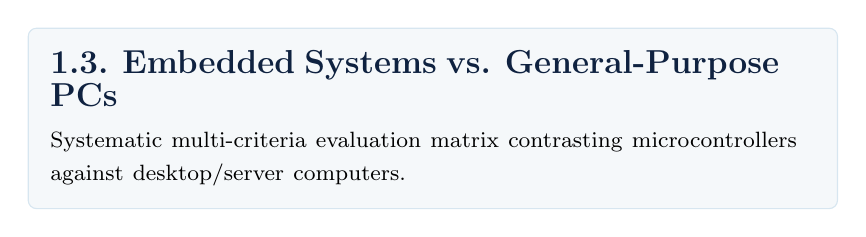
\begin{tikzpicture}
        \node[fill=cardbg, draw=bordergray, rounded corners=3pt, text width=0.45\paperwidth, inner sep=8pt] {
          \textbf{\fontsize{13}{15}\selectfont\color{darknavy}1.3. Embedded Systems vs. General-Purpose PCs}\\[0.1cm]
          {\footnotesize Systematic multi-criteria evaluation matrix contrasting microcontrollers against desktop/server computers.}
        };
      \end{tikzpicture}\\[0.25cm]
      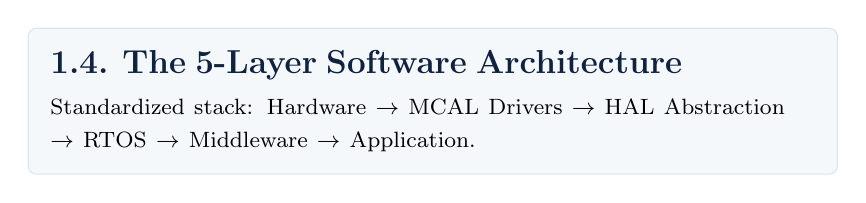
\begin{tikzpicture}
        \node[fill=cardbg, draw=bordergray, rounded corners=3pt, text width=0.45\paperwidth, inner sep=8pt] {
          \textbf{\fontsize{13}{15}\selectfont\color{darknavy}1.4. The 5-Layer Software Architecture}\\[0.1cm]
          {\footnotesize Standardized stack: Hardware $\rightarrow$ MCAL Drivers $\rightarrow$ HAL Abstraction $\rightarrow$ RTOS $\rightarrow$ Middleware $\rightarrow$ Application.}
        };
      \end{tikzpicture}
    \end{column}
  \end{columns}

  \vspace{0.35cm}
  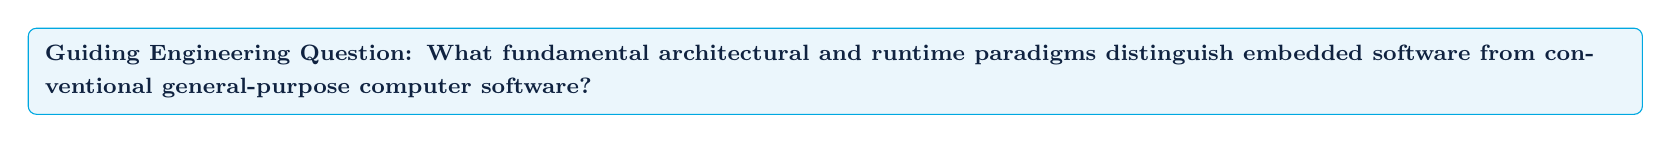
\begin{tikzpicture}
    \node[fill=calloutbg, draw=bannerblue, rounded corners=3pt, text width=0.93\paperwidth, inner sep=6pt] {
      \textbf{\footnotesize\color{darknavy}Guiding Engineering Question: What fundamental architectural and runtime paradigms distinguish embedded software from conventional general-purpose computer software?}
    };
  \end{tikzpicture}
\end{frame}

% ============================================================================
% SLIDE 3: 1.1 DEFINITION & TRIAD NATURE
% ============================================================================
\begin{frame}[t]
  \slidetitle{1.1. Embedded System Definition \& Nature}
  \begin{columns}[c]
    \begin{column}{0.46\textwidth}
      \centering
      \includegraphics[width=\linewidth,height=0.62\textheight,keepaspectratio]{images/fig_1_1_typical_system.jpg}\\[0.15cm]
      {\footnotesize\color{black!70}\textit{Figure 1.1: Architecture of a Typical Embedded System.}}
    \end{column}
    \begin{column}{0.52\textwidth}
      \raggedright
      \begin{itemize}
        \item \textbf{Standard Definition:} A specialized computing system integrated inside a host equipment or machinery, engineered strictly to execute pre-defined dedicated functions.
        \item \textbf{The 3-Element Triad:} Inseparable co-design between \textbf{Computation Engine} (Hardware) --- \textbf{Processing Logic} (Firmware) --- \textbf{Physical World Interaction} (Sensors/Actuators).
        \item \textbf{Design Objective:} Fulfill dedicated tasks under strict physical constraints: deterministic timing, ultra-low power, compact footprint, high MTBF, and low unit cost.
        \item \textbf{Core Distinction:} Fundamentally diverges from PCs: eliminates general-purpose software bloat in favor of deep optimization for a singular dedicated workload.
        \item \textbf{Industrial Edge Example:} Environmental Telemetry Station: Continuous sensing, on-device wildfire/anomaly detection, and 24/7 telemetry.
      \end{itemize}
    \end{column}
  \end{columns}
\end{frame}

% ============================================================================
% SLIDE 4: 1.1 HARDWARE ARCHITECTURE & SUBSYSTEMS
% ============================================================================
\begin{frame}[t]
  \slidetitle{1.1. Hardware Architecture \& Subsystems}
  \begin{columns}[c]
    \begin{column}{0.46\textwidth}
      \centering
      \includegraphics[width=\linewidth,height=0.62\textheight,keepaspectratio]{images/fig_1_1_2_hardware.jpg}\\[0.15cm]
      {\footnotesize\color{black!70}\textit{Figure 1.2: Hardware Subsystems of an Embedded Device.}}
    \end{column}
    \begin{column}{0.52\textwidth}
      \raggedright
      \sectionheader{Core Hardware Subsystems (MCU):}
      \begin{itemize}
        \item \textbf{Processing Core (MCU/MPU):} Silicon microcontroller integrating CPU, hardware timers, DMA controllers, and low-latency NVIC.
        \item \textbf{Memory Hierarchy:} Embedded \textbf{Flash Memory} for non-volatile firmware; tight on-chip \textbf{SRAM} for execution stack, heap, and peripheral buffers.
        \item \textbf{Physical Transducers:} High-precision \textbf{Sensors} paired with robust \textbf{Actuators} (relays, buzzers, solenoid valves, motor drivers).
        \item \textbf{Communication Buses:} Local serial interfaces (\textbf{UART, SPI, I2C, CAN}) alongside networked transceivers (\textbf{Ethernet, Wi-Fi, Cellular}).
        \item \textbf{Power \& Protection:} Integrated \textbf{LDO} regulators, Brown-Out Detector (\textbf{BOD}), and hardware \textbf{Watchdog Timers}.
      \end{itemize}
    \end{column}
  \end{columns}
\end{frame}

% ============================================================================
% SLIDE 5: 1.1 EMBEDDED NATURE & EDGE COMPUTING IN IOT
% ============================================================================
\begin{frame}[t]
  \slidetitle{1.1. Embedded Nature \& Edge Computing in IoT}
  \begin{columns}[c]
    \begin{column}{0.46\textwidth}
      \centering
      \includegraphics[width=\linewidth,height=0.62\textheight,keepaspectratio]{images/fig_1_1_3_edge.png}\\[0.15cm]
      {\footnotesize\color{black!70}\textit{Figure 1.3: Embedded Edge Node in Cloud-IoT Topology.}}
    \end{column}
    \begin{column}{0.52\textwidth}
      \raggedright
      \begin{itemize}
        \item \textbf{The `Embedded' Nature:} Deeply encapsulated within host equipment; users interact solely via high-level HMIs or cloud dashboards; requires bare-metal register manipulation.
        \item \textbf{Frontline IoT Edge Node:} Serves as the vital physical bridge collecting telemetry directly at the sensor layer and driving deterministic physical actuation.
        \item \textbf{On-Device Edge Computing:} Performs local digital filtering, anomaly classification, and lightweight inference at the edge, drastically reducing cloud bandwidth and latency.
        \item \textbf{Disconnection Resilience:} Operates 100\% autonomously during WAN network blackouts; triggers local safety cutoffs independently without cloud reliance.
        \item \textbf{Non-Volatile Data Buffering:} Retains critical telemetry on local SD/Flash memory during signal loss and automatically synchronizes upon reconnection.
      \end{itemize}
    \end{column}
  \end{columns}
\end{frame}

% ============================================================================
% SLIDE 6: 1.2 DEDICATED FUNCTIONALITY & RESOURCE CONSTRAINTS
% ============================================================================
\begin{frame}[t]
  \slidetitle{1.2. Dedicated Functionality \& Resource Constraints}
  \begin{columns}[c]
    \begin{column}{0.46\textwidth}
      \centering
      \includegraphics[width=\linewidth,height=0.62\textheight,keepaspectratio]{images/fig_1_2_characteristics.jpg}\\[0.15cm]
      {\footnotesize\color{black!70}\textit{Figure 1.4: Multi-dimensional Constraints in Embedded Design.}}
    \end{column}
    \begin{column}{0.52\textwidth}
      \raggedright
      \sectionheader{Specialization vs. Constraints:}
      \begin{itemize}
        \item \textbf{Application-Specific Co-Design:} Hardware and firmware are strictly trimmed to the target workload $\rightarrow$ minimizes BOM unit cost and eliminates software bloat.
        \item \textbf{Engineered Trade-off:} Sacrifices generic software flexibility; substantial functional modifications necessitate PCB and schematic redesign.
        \item \textbf{Scarce Non-Volatile Flash:} Constrained to tens of KB to few MB (vs. hundreds of GB SSD on PCs) $\rightarrow$ demands aggressive code footprint minimization.
        \item \textbf{Extremely Tight SRAM:} Limited to 16 KB -- 512 KB $\rightarrow$ \textbf{dynamic heap allocation (\texttt{malloc}) is strictly prohibited} to prevent heap fragmentation; static allocation is mandatory.
        \item \textbf{Clock Speed \& Pinout:} Conservative MHz clock rates to conserve battery; tightly budgeted GPIO pinout requires pin multiplexing.
      \end{itemize}
    \end{column}
  \end{columns}
\end{frame}

% ============================================================================
% SLIDE 7: 1.2 REAL-TIME DETERMINISM & SYSTEM RELIABILITY
% ============================================================================
\begin{frame}[t]
  \slidetitle{1.2. Real-Time Determinism \& System Reliability}
  \raggedright
  \begin{columns}[t]
    \begin{column}{0.48\textwidth}
      \sectionheader{Real-Time Determinism \& Deadlines}
      \begin{itemize}
        \item \textbf{Correctness Criteria:} System correctness requires \textbf{both} logical accuracy AND completion strictly before defined \textbf{Deadlines}.
        \item \textbf{Hard Real-Time:} Missing a deadline causes catastrophic destruction or loss of human life (\textit{airbags, ABS braking, medical ventilators}).
        \item \textbf{Soft Real-Time:} Deadline misses degrade Quality of Service without catastrophic harm (\textit{UI display refresh, periodic logging}).
        \item \textbf{Deterministic Timing:} Interrupt latency and task execution times must have mathematical upper bounds; zero tolerance for unbounded jitter.
        \item \textbf{Architectural Support:} Enforced via low-latency NVIC and preemptive priority RTOS scheduling.
      \end{itemize}
    \end{column}
    \begin{column}{0.48\textwidth}
      \sectionheader{Autonomous Reliability \& Self-Healing}
      \begin{itemize}
        \item \textbf{Continuous 24/7/365 Uptime:} Must operate unattended for decades without human manual intervention or reboot.
        \item \textbf{Hardware Watchdog (WDT):} Independent free-running counter resets the MCU automatically if firmware enters a deadlock or infinite loop.
        \item \textbf{Brown-Out Detector (BOD):} Continually monitors supply voltage droop, forcing safe reset before Flash memory is corrupted.
        \item \textbf{Cyclic Redundancy Checks (CRC):} Hardware CRC engine verifies Flash code integrity and communication packet validity.
        \item \textbf{Fail-Safe Defaults:} Automatic fallback into safe benign states (\textit{opening relays, sounding alarms}) upon critical faults.
      \end{itemize}
    \end{column}
  \end{columns}
\end{frame}

% ============================================================================
% SLIDE 8: 1.2 POWER EFFICIENCY, SECURITY & MAINTENANCE
% ============================================================================
\begin{frame}[t]
  \slidetitle{1.2. Power Efficiency, Security \& Maintenance}
  \raggedright
  \begin{columns}[t]
    \begin{column}{0.48\textwidth}
      \sectionheader{Ultra-Low Power Optimization}
      \begin{itemize}
        \item \textbf{Deep Sleep States:} Advanced low-power modes (Sleep, Standby, Deep Software Standby) dropping quiescent current to microamperes ($\mu\text{A}$).
        \item \textbf{Interrupt-Driven Wakeup:} CPU core remains powered down, waking up solely upon external sensor edge interrupts or periodic RTC timers.
        \item \textbf{Autonomous DMA Transfers:} Direct Memory Access transfers peripheral data to RAM buffers without CPU intervention, maximizing sleep duty cycles.
        \item \textbf{Energy Harvesting:} Supports ultra-low-power duty cycles compatible with solar, thermal, and RF energy-harvesting nodes.
      \end{itemize}
    \end{column}
    \begin{column}{0.48\textwidth}
      \sectionheader{Embedded Security \& Maintenance}
      \begin{itemize}
        \item \textbf{Hardware Secure Boot:} Silicon cryptographic engine validates digital signatures (RSA/ECC) of firmware before allowing boot execution.
        \item \textbf{Arm TrustZone Isolation:} Partitions memory and peripherals into Secure and Non-Secure domains, isolating encryption keys from user code.
        \item \textbf{Line-Rate Encryption:} Hardware-accelerated AES, SHA-256, and ECC engines enable secure TLS/DTLS encryption for cloud telemetry.
        \item \textbf{Dual-Bank Flash OTA:} Downloads and stages new firmware images into secondary Flash bank without downtime; automated rollback on failure.
      \end{itemize}
    \end{column}
  \end{columns}
\end{frame}

% ============================================================================
% SLIDE 9: 1.3 EMBEDDED SYSTEMS VS. GENERAL-PURPOSE PCS
% ============================================================================
\begin{frame}[t]
  \slidetitle{1.3. Embedded Systems vs. General-Purpose PCs}
  \begin{columns}[c]
    \begin{column}{0.46\textwidth}
      \centering
      \includegraphics[width=\linewidth,height=0.62\textheight,keepaspectratio]{images/fig_1_3_gpc_vs_embedded.jpg}\\[0.15cm]
      {\footnotesize\color{black!70}\textit{Figure 1.5: Paradigm Comparison: General-Purpose PC vs. Embedded System.}}
    \end{column}
    \begin{column}{0.52\textwidth}
      \raggedright
      \begin{itemize}
        \item \textbf{Specialization vs. Versatility:} General-Purpose Computers (GPC) run arbitrary multi-user software, office suites, and gaming. Embedded systems are deeply pruned for one dedicated lifecycle workload.
        \item \textbf{Monolithic SoC/MCU Integration:} Embedded MCUs integrate CPU, SRAM, Flash ROM, ADC/DAC, timers, and serial controllers on a single silicon die. PCs rely on discrete motherboards with socketed CPUs, off-chip RAM sticks, and SSD drives.
        \item \textbf{Environmental Robustness:} Embedded systems survive extreme industrial temperatures (-40°C to +85°C/125°C), high vibration, dust, and electrical noise. PCs require climate-controlled indoor environments and active fan cooling.
        \item \textbf{Cost \& Unit Optimization:} MCU Bill-of-Materials cost is measured in single-digit dollars for mass production, whereas PC platforms cost hundreds to thousands of dollars.
      \end{itemize}
    \end{column}
  \end{columns}
\end{frame}

% ============================================================================
% SLIDE 10: 1.3 DETAILED TECHNICAL COMPARISON MATRIX
% ============================================================================
\begin{frame}[t]
  \slidetitle{1.3. Detailed Technical Comparison Matrix}
  \centering
  \vspace{-0.1cm}
  \scriptsize
  \renewcommand{\arraystretch}{1.18}
  \begin{tabularx}{0.96\textwidth}{>{\raggedright\arraybackslash\bfseries\color{darknavy}}p{2.2cm} >{\raggedright\arraybackslash}X >{\raggedright\arraybackslash}X}
    \toprule
    \rowcolor{bannerblue}
    \color{white}\textbf{Evaluation Metric} & \color{white}\textbf{Embedded Systems (MCU-based)} & \color{white}\textbf{General-Purpose Computers (PC-based)} \\
    \midrule
    Design Objective & Dedicated, deeply optimized for a single mission & Versatile, executes arbitrary concurrent user applications \\
    \rowcolor{rowalt}
    Processor Core & Low-power MCU (e.g., ARM Cortex-M), SoC, DSP (MHz) & High-speed multi-core CPU (x86/x64, GHz), discrete GPU \\
    Memory Hierarchy & Flash: 32 KB -- 4 MB; SRAM: 8 KB -- 1 MB (On-chip) & RAM: 8 GB -- 64+ GB; Storage: 512 GB -- Multiple TB SSD \\
    \rowcolor{rowalt}
    Operating System & Bare-metal firmware, Hard RTOS (\textit{FreeRTOS, Zephyr}) & General-Purpose OS (\textit{Windows, Linux, macOS}) \\
    Timing Constraints & Deterministic hard/soft real-time; bounded $\mu$s latency & Best-effort execution; non-deterministic task scheduling \\
    \rowcolor{rowalt}
    Power Consumption & Ultra-low power (mW to $\mu$A); multi-year battery & High power draw (50W -- 500W+); continuous AC mains \\
    Operating Environment & Harsh industrial (-40°C to 85°C), vibration, dust & Benign indoor climate; office/datacenter environments \\
    \rowcolor{rowalt}
    Maintenance Lifecycle & Secure remote OTA firmware; decades-long operational life & Frequent OS patches, dynamic package installations \\
    \bottomrule
  \end{tabularx}

  \vspace{0.2cm}
  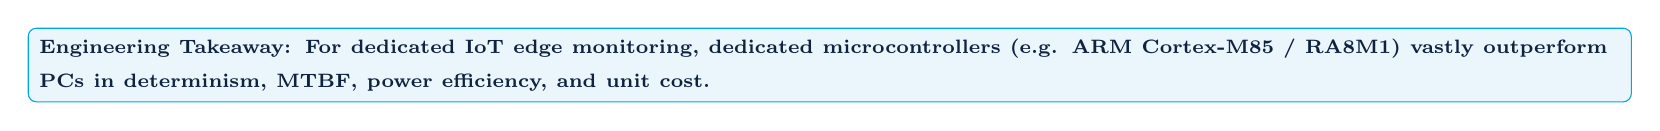
\begin{tikzpicture}
    \node[fill=calloutbg, draw=bannerblue, rounded corners=3pt, text width=0.93\paperwidth, inner sep=4pt] {
      \textbf{\scriptsize\color{darknavy}Engineering Takeaway: For dedicated IoT edge monitoring, dedicated microcontrollers (e.g. ARM Cortex-M85 / RA8M1) vastly outperform PCs in determinism, MTBF, power efficiency, and unit cost.}
    };
  \end{tikzpicture}
\end{frame}

% ============================================================================
% SLIDE 11: 1.4 THE 5-LAYER SOFTWARE ARCHITECTURE
% ============================================================================
\begin{frame}[t]
  \slidetitle{1.4. The 5-Layer Embedded Software Architecture}
  \begin{columns}[c]
    \begin{column}{0.46\textwidth}
      \centering
      \includegraphics[width=\linewidth,height=0.62\textheight,keepaspectratio]{images/fig_1_4_layered_arch.jpg}\\[0.15cm]
      {\footnotesize\color{black!70}\textit{Figure 1.6: Standard 5-Layer Embedded Software Stack.}}
    \end{column}
    \begin{column}{0.52\textwidth}
      \raggedright
      \begin{itemize}
        \item \textbf{Separation of Concerns:} Each architectural tier encapsulates specific functional responsibilities, hiding lower-level hardware quirks from upper layers.
        \item \textbf{Hardware Decoupling:} Application logic never manipulates raw chip registers; all hardware interactions pass through standardized APIs.
        \item \textbf{Concurrent Engineering \& Host Testing:} Hardware schematics and software develop in parallel; allows extensive Unit Testing natively on host PCs.
        \item \textbf{Silicon Portability:} When migrating to an alternative MCU vendor, only the MCAL/HAL drivers are rewritten---preserving \textbf{100\% of Middleware and Application code}.
        \item \textbf{Extensibility:} Modifying hardware components (\textit{e.g., swapping an analog sensor for an I2C sensor}) requires zero changes to core business rules.
      \end{itemize}
    \end{column}
  \end{columns}
\end{frame}

% ============================================================================
% SLIDE 12: 1.4.1 – 1.4.2 HARDWARE LAYER & MCAL / HAL
% ============================================================================
\begin{frame}[t]
  \slidetitle{1.4.1 -- 1.4.2. Hardware Layer \& MCAL / HAL}
  \raggedright
  \begin{columns}[t]
    \begin{column}{0.48\textwidth}
      \sectionheader{Physical Hardware Layer}
      \begin{itemize}
        \item \textbf{Target Silicon:} MCU silicon (e.g., Renesas RA8M1 / Cortex-M85), analog front-ends, relay drivers, communication transceivers.
        \item \textbf{PCB Layout Integrity:} Physical trace routing directly dictates Signal-to-Noise Ratio (SNR), ADC sampling precision, and parasitic leakage currents.
        \item \textbf{Hardware Robustness:} In-line PTC resettable fuses, TVS suppression diodes, and galvanic isolation prevent field electrical destruction.
        \item \textbf{Engineering Reality:} Silicon layout bugs and hardware flaws cannot be solved by software patches alone---demands rigorous design validation.
      \end{itemize}
    \end{column}
    \begin{column}{0.48\textwidth}
      \sectionheader{MCAL vs. HAL Driver Layers}
      \begin{itemize}
        \item \textbf{MCAL (Microcontroller Abstraction):} Hardware-dependent register manipulation; configures internal silicon clocks, pin multiplexing, interrupt routing, and DMA channels.
        \item \textbf{HAL (Hardware Abstraction Layer):} Vendor-neutral API abstraction wrapping register complexity into uniform C calls (\texttt{HAL\_GPIO\_WritePin()}, \texttt{HAL\_ADC\_Read()}).
        \item \textbf{Device Driver Interface:} Provides standard bus interfaces allowing external sensor/actuator drivers to operate seamlessly across different chips.
        \item \textbf{Portability Boundary:} Decouples silicon-specific CMSIS headers from higher-level middleware and application stacks.
      \end{itemize}
    \end{column}
  \end{columns}
\end{frame}

% ============================================================================
% SLIDE 13: 1.4.3 REAL-TIME OPERATING SYSTEM (RTOS LAYER)
% ============================================================================
\begin{frame}[t]
  \slidetitle{1.4.3. Real-Time Operating System (RTOS Layer)}
  \raggedright
  \begin{columns}[t]
    \begin{column}{0.48\textwidth}
      \sectionheader{Preemptive Multitasking vs. Super-Loop}
      \begin{itemize}
        \item \textbf{Super-Loop Pitfalls:} Sequential \texttt{while(1)} polling suffers catastrophic latency blockage when long I/O tasks (\textit{e.g., TCP network handshakes}) stall the CPU.
        \item \textbf{Preemptive Priority Scheduling:} Critical high-priority tasks (\textit{e.g., fire detection, over-temperature alarm}) preempt the CPU within microseconds upon interrupt.
        \item \textbf{Deterministic Software Timers:} Non-blocking software timers drive periodic sensor acquisitions with millisecond determinism.
        \item \textbf{Tickless Low-Power Idle:} Automatically transitions the MCU core into deep sleep whenever all tasks are blocked in wait states.
      \end{itemize}
    \end{column}
    \begin{column}{0.48\textwidth}
      \sectionheader{IPC \& Resource Synchronization}
      \begin{itemize}
        \item \textbf{Message Queues:} Safe FIFO message queues pass sensor telemetry to processing tasks without memory corruption or locks.
        \item \textbf{Mutexes \& Semaphores:} Guard shared communication buses (\textit{I2C, SPI, UART}) against race conditions and priority inversions.
        \item \textbf{Task Priority Hierarchy:} Emergency Safety Alarms (High) $\rightarrow$ Sensor Filtering (Medium) $\rightarrow$ Cloud MQTT Telemetry (Low).
        \item \textbf{Leading Industrial RTOS:} \textbf{FreeRTOS} (ubiquitous, minimal footprint), \textbf{Zephyr RTOS} (modular, modern IoT stack), \textbf{Azure RTOS / ThreadX}.
      \end{itemize}
    \end{column}
  \end{columns}
\end{frame}

% ============================================================================
% SLIDE 14: 1.4.4 MIDDLEWARE & SYSTEM SERVICES LAYER
% ============================================================================
\begin{frame}[t]
  \slidetitle{1.4.4. Middleware \& System Services Layer}
  \raggedright
  \begin{columns}[t]
    \begin{column}{0.48\textwidth}
      \sectionheader{IoT Networking \& Protocol Stacks}
      \begin{itemize}
        \item \textbf{Embedded TCP/IP Stack:} Lightweight network stacks (\textbf{LwIP}, FreeRTOS-Plus-TCP) powering low-overhead Ethernet and Wi-Fi connectivity.
        \item \textbf{MQTT Protocol:} Lightweight Publish/Subscribe messaging protocol minimizing transmission packet overhead and radio active time.
        \item \textbf{CoAP \& HTTP Micro-Servers:} Embedded micro-web servers for on-site device commissioning, status diagnostics, and RESTful APIs.
        \item \textbf{DHCP \& DNS Clients:} Automated IP dynamic configuration and central cloud hostname resolution over dynamic local networks.
      \end{itemize}
    \end{column}
    \begin{column}{0.48\textwidth}
      \sectionheader{Security, Storage \& Maintenance}
      \begin{itemize}
        \item \textbf{Cryptographic Library (MbedTLS):} Implements industry-grade TLS 1.3 / DTLS encryption, safeguarding telemetry against eavesdropping and MITM attacks.
        \item \textbf{Embedded File System (FatFS):} Hardware-independent FAT12/16/32 and exFAT implementation for local microSD and external SPI Flash storage.
        \item \textbf{Robust OTA Engine:} Handles remote firmware download, cryptographic hash validation (SHA-256), and dual-bank Flash staging.
        \item \textbf{Diagnostics \& Logging:} Tracks runtime CPU load, stack watermarks, memory leaks, and records multi-level error logs for post-mortem analysis.
      \end{itemize}
    \end{column}
  \end{columns}
\end{frame}

% ============================================================================
% SLIDE 15: 1.4.5 APPLICATION LAYER & DOMAIN LOGIC
% ============================================================================
\begin{frame}[t]
  \slidetitle{1.4.5. Application Layer \& Domain Logic}
  \raggedright
  \begin{columns}[t]
    \begin{column}{0.48\textwidth}
      \sectionheader{Core Domain Tasks \& Signal Processing}
      \begin{itemize}
        \item \textbf{Periodic Sampling:} Orchestrates multi-sensor data acquisition (ambient temperature, relative humidity, VOC/toxic gas, structural vibration).
        \item \textbf{Digital Signal Processing:} Implements Moving Average or Kalman filters to eliminate electrical noise spikes and sensor drift.
        \item \textbf{Threshold Evaluation:} Classifies environmental health across multi-tiered levels: Normal $\rightarrow$ Warning $\rightarrow$ Critical Alarm.
        \item \textbf{Autonomous Emergency Actuation:} Drives safety actuators immediately upon anomaly detection (\textit{opening relays, running fans, sirens}).
        \item \textbf{Telemetry Serialization:} Encodes validated telemetry into compact standard formats (\textit{JSON, CBOR, Protocol Buffers}).
      \end{itemize}
    \end{column}
    \begin{column}{0.48\textwidth}
      \sectionheader{Design Decoupling \& Host Testability}
      \begin{itemize}
        \item \textbf{Total Hardware Independence:} Pure business logic interacts strictly through generic domain APIs (\texttt{get\_sensor\_data()}, \texttt{trigger\_alarm()}).
        \item \textbf{Transducer Modularity:} Replacing an analog sensor with an I2C sensor leaves 100\% of threshold comparison logic completely untouched.
        \item \textbf{Host-Based Simulation:} Entire application state machine compiles and runs on a host PC using simulated sensor streams for rapid verification.
        \item \textbf{Finite State Machine (FSM):} Structured as deterministic states: Boot $\rightarrow$ Normal Operation $\rightarrow$ Warning $\rightarrow$ Emergency Fault.
      \end{itemize}
    \end{column}
  \end{columns}
\end{frame}

% ============================================================================
% SLIDE 16: CHAPTER SUMMARY & TRANSITION TO CHAPTER II
% ============================================================================
\begin{frame}[t]
  \slidetitle{Chapter I Summary \& Transition to Chapter II}
  \raggedright
  \vspace{0.05cm}

  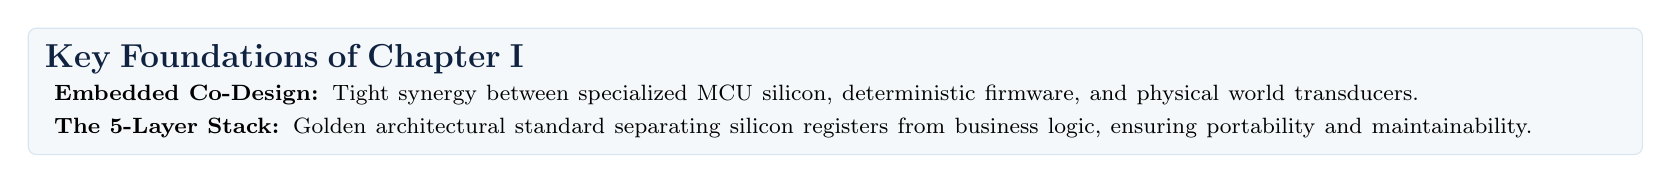
\begin{tikzpicture}
    \node[fill=cardbg, draw=bordergray, rounded corners=3pt, text width=0.93\paperwidth, inner sep=6pt] {
      \textbf{\fontsize{12}{14}\selectfont\color{darknavy}Key Foundations of Chapter I}\\[0.08cm]
      \footnotesize
      $\blacktriangleright$ \textbf{Embedded Co-Design:} Tight synergy between specialized MCU silicon, deterministic firmware, and physical world transducers.\\
      $\blacktriangleright$ \textbf{The 5-Layer Stack:} Golden architectural standard separating silicon registers from business logic, ensuring portability and maintainability.
    };
  \end{tikzpicture}\\[0.2cm]

  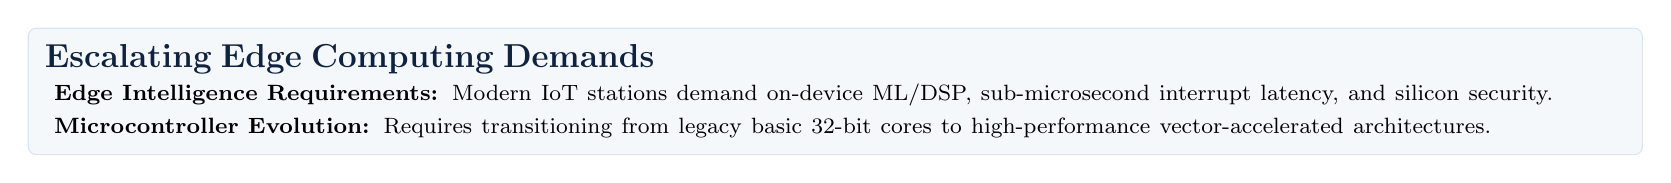
\begin{tikzpicture}
    \node[fill=cardbg, draw=bordergray, rounded corners=3pt, text width=0.93\paperwidth, inner sep=6pt] {
      \textbf{\fontsize{12}{14}\selectfont\color{darknavy}Escalating Edge Computing Demands}\\[0.08cm]
      \footnotesize
      $\blacktriangleright$ \textbf{Edge Intelligence Requirements:} Modern IoT stations demand on-device ML/DSP, sub-microsecond interrupt latency, and silicon security.\\
      $\blacktriangleright$ \textbf{Microcontroller Evolution:} Requires transitioning from legacy basic 32-bit cores to high-performance vector-accelerated architectures.
    };
  \end{tikzpicture}\\[0.2cm]

  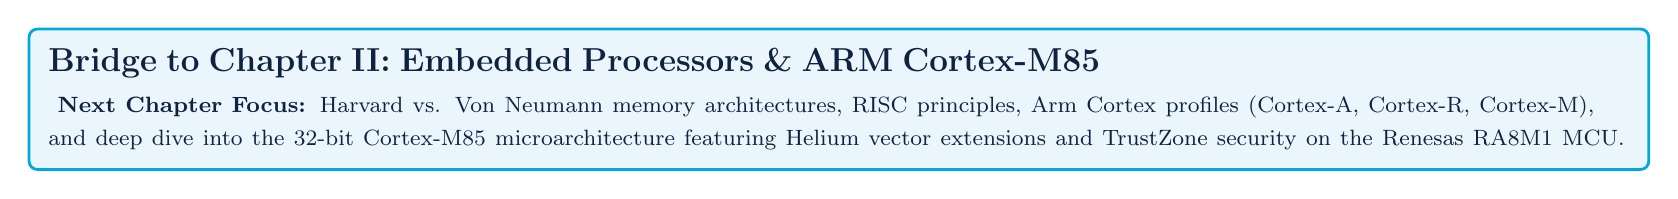
\begin{tikzpicture}
    \node[fill=calloutbg, draw=bannerblue, line width=1pt, rounded corners=3pt, text width=0.93\paperwidth, inner sep=7pt] {
      \textbf{\fontsize{13}{15}\selectfont\color{darknavy}Bridge to Chapter II: Embedded Processors \& ARM Cortex-M85}\\[0.1cm]
      \footnotesize\color{darknavy}
      $\blacktriangleright$ \textbf{Next Chapter Focus:} Harvard vs. Von Neumann memory architectures, RISC principles, Arm Cortex profiles (Cortex-A, Cortex-R, Cortex-M), and deep dive into the 32-bit Cortex-M85 microarchitecture featuring Helium vector extensions and TrustZone security on the Renesas RA8M1 MCU.
    };
  \end{tikzpicture}
\end{frame}

\end{document}
